\subsection{Rogue APs}
\label{subsec:rogue}

Rogue Access Points (RAPs) are unauthorized APs that are deployed within an
enterprise network \cite{beyah-rogueap11}.  While RAPs can increase exposure
to potential security vulnerabilities, for the purpose of this paper we are concerned
with the introduction of additional RF interference and new complexities with regards
to spectrum management. Previous
works~\cite{bahl2006enhancing,ma2008hybrid,wei2007passive} have focused on RAP
detection viewing any RAP as a potential security vulnerability.  In reality, however, 
many RAPs are set up by users who have authorized access to the campus wireless 
network yet are not satisfied with its performance. In contrast to the existing literature,
we focus on what we dub \emph{benign RAPs}, namely those RAPs that are not
intentionally malicious.  The client-centric view afforded by our datasets allow us to explore 
several key questions that include: (1) To what extent are benign RAPs actually benign 
to the broader campus population, ex. how do RAPs impact legitimate campus network
users? (2) Are the performance improvements of RAPs actually better for non-trivial
populations and what implications does this have for campus network management?

% Edits: The prior works do not really distinguish between malicious versus benign
%  APs as there really is no such thing as a benign rogue AP.  Edited the text to bring
% along that mindset

% Changed most to many to soften the text a bit

\subsubsection{Impact of RAPs}
\label{subsec:rap_impact}

\begin{figure}[t]
  \centering
  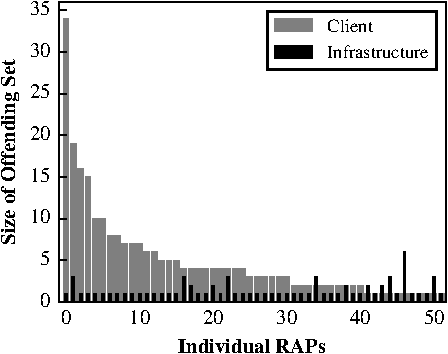
\includegraphics[width=\columnwidth]{./figures/CampusRAPImpact.pdf}
  \caption{\textbf{Client vs. Infrastructure Offending Set Size of
    the RAPs.} RAPs are sorted in descending order of client measured offending
  set size.}
  \label{fig:rap_impact}
  \vspace*{\aftercaptiongap}
\end{figure}

Intrinsically, RAPs compete for the same spectrum with the campus APs. RAPs may be
well-placed, choosing largely orthogonal channels to the existing campus network or
poorly configured with little to no oversight with regards to the legitimate network.  
To quantify the impact of RAPs on campus wireless network, we define the 
\textit{offending set} of an individual RAP ($RAP_i$) as the set of all campus APs 
that suffer interference from $RAP_i$ and hence are
``offended'' by $RAP_i$.  Hence, the size of the offending 
set can be thought of as a coarse benchmark for gauging the severity of interference
created by $RAP_i$.  While the benchmark does not fully capture nuance of interference
entirely, we believe it presents an intuitive metric and we discuss several alternatives
in Section~\ref{subsec:rap_discussion}.
   
% There is not a may not capture assertion, it really does not catch the nuance of the degree
% of orthogonality when a channel is interfering along with distance.  Thought about doing
% the offending set as OS_i but that is ugly.  

The simplest mechanism to generate the listing of RAPs can be gleaned from the underlying
campus wireless network reporting infrastructure whereby the population of the offending
set is built entirely through AP-side observations.  However, as shown earlier in
Section~\ref{subsec:client_conflict}, the interference range of a RAP can extend far
beyond its immediate campus AP neighbors due to hidden terminal effects.  As a result,
the campus network user perception of RAP interference may vary significantly from the
infrastructure view (both with positive and negative effects).  

We now quantify such differences by building the client-centric offending set for each
RAP ($RAP_i$).  For a scan result $R=(RAP_1,
RAP_2,\ldots,RAP_m, AP_1, \ldots, AP_n)$ reported during a \wifi{} session with
campus AP $AP_c$, where $RAP_i (1 \le i \le m)$ is a rogue AP and $AP_j(1 \le j
\le n)$ is a campus AP, we add $AP_c$ to each of the $RAP_i$'s offending
set if $RAP_i$ would be interfering with $AP_c$.  

%, since each $RAP_i$ causes either collisions to $AP_c$'s downlink packets,
%or extra backoff delay for uplink packets from $AP_c$'s clients.

Figure~\ref{fig:rap_impact} shows the offending set sizes comparison for the 52
RAPs detected both in \ubscan{} dataset and campus RAP reports. As expected, most
RAPs cause interferences to far more campus APs than the infrastructure can tell.
More interestingly, when sorting the RAPs by their offending set size, several of
the ranking of the RAPs are different in the two offending set construction methods. 
That is, from infrastructure RAP reports, network operators may think $RAP_i$ causes more
interference than $RAP_j$, while $RAP_j$ in fact offends more campus APs than
$RAP_i$ from the perspective of the client. More precisely, for RAP pairs, $\langle RAP_i,
RAP_j \rangle$, we say the offending set constructions \textit{agree} on this
pair if the two RAPs are ranked in same order, otherwise, they \textit{disagree}
on the severity of the two RAPs. Among all $C_{52}^{51}=1326$ RAP pairs in
Figure~\ref{fig:rap_impact}, we found the client and infrastructure constructed
offending sets disagree with each other on 549 (41\%) pairs.

\subsubsection{Implications of RAPs}
\label{subsec:rap_implicaton}

\begin{figure}[t]
  \centering
  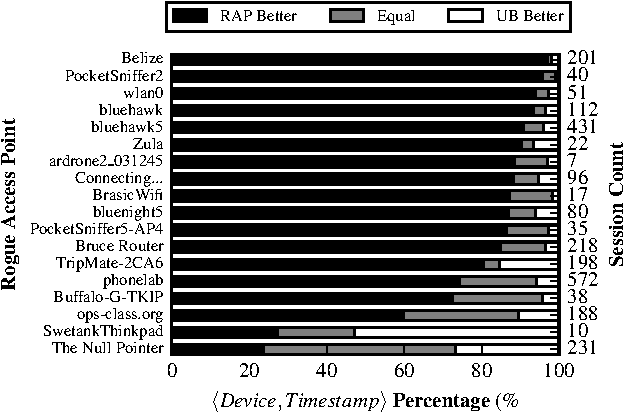
\includegraphics[width=\columnwidth]{./figures/RAPSessionCampusRSSIFigure.pdf}
  \caption{\textbf{Campus AP v. RAP Signal Strength.} Comparisons are
  performed during \wifi{} sessions with the listed RAP, and RSSI values
  within 5~dBm are considered equivalent.}
  \label{fig:rap_session_ub_signal}
\end{figure}

From a full disclosure perspective, it is important to note that multiple coauthors of the
paper operate RAPs for (what we believe to be) legitimate and justifiable reasons.
As such, we are certainly more sympathetic to the presence of RAPs. Therefore, 
we now reverse the study and ask the question: \textit{do RAPs really provide 
better coverage than campus APs?}

In the \ubscan{} dataset, we found \num{2763} \wifi{} sessions with 26 RAPs from
44 devices. For each scan result reported during session with a RAP, we
compare the signal strength of the associated RAP ($RSSI_{rogue}$) versus the
best RSSI from campus APs ($RSSI_{campus}$). If $|RSSI_{rogue}-RSSI_{campus}|
< 5$dBm, we classify them as equal, to tolerate possible RSSI fluctuations.
Otherwise the AP with larger RSSI is better. We then classify each
unique $\langle device, timestamp \rangle$ pair of each scan result into one of 
three categories (RAP Better, Equal, UB Better).  

Figure~\ref{fig:rap_session_ub_signal} shows the comparison of 18 RAPs that
provided at least 10 \wifi{} sessions to \PhoneLab{} participants. In most
cases, the RAPs do seem to be providing a better signal than the user would
have achieved using the campus network. In such cases, RAPs may have
accurately identified weak coverage spots in the campus network and should be
considered during future spatial planning. Conversely, some RAPs (e.g.,
\texttt{The Null Pointer}) did not provide significantly better signal
strength for the \PhoneLab{} participants who connected to those RAPs,
indicating they should have used the campus network.

\subsubsection{Discussion}
\label{subsec:rap_discussion}

As noted earlier, the size of the offending set may not be the only factor that determines
the severity of a given RAP.  Notably, a heavily loaded RAP consumes significantly more
airtime and is much more likely to cause interference with campus APs over an idle RAP.  
Such load information on the RAP, however, cannot be easily obtained outside of using
dedicated packet sniffers at the right time and right location.  Furthermore, not all 
interference is created equal as the channel separation between the
RAP and campus infrastructure will significantly impact interference.  A rogue AP may only
slightly interfere with the infrastructure APs at that particular point in space.  

Finally, one key impact that is not directly captured by interference is the extent to which
the presence of RAPs constrain the solution space afforded to the infrastructure for
channel selection.  While an aggressive infrastructure could ignore scan results, a 
more adaptive infrastructure might find certain channels no longer available which in
turn may lead to a sub-optimal deployment or increased channel interference amongst
legitimate nodes in the campus infrastructure.      

%Another possible metric to consider the total load in the RAP's
%offending set: the more busy the offended campus APs, the more interferences the
%RAP may potentially cause.
